% Intended LaTeX compiler: pdflatex
\documentclass[dvipdfmx,10pt,presentation]{beamer}
\usepackage{amsmath, amssymb, bm}
\usepackage[utf8]{inputenc}
\usepackage{indentfirst}
\usepackage[normalem]{ulem}
\usepackage{longtable}
\usepackage{minted}
\usepackage{fancyvrb}
\usetheme{Berlin}
\usepackage[utf8]{inputenc}
\usepackage[T1]{fontenc}
\usepackage{graphicx}
\usepackage{grffile}
\usepackage{longtable}
\usepackage{wrapfig}
\usepackage{rotating}
\usepackage[normalem]{ulem}
\usepackage{amsmath}
\usepackage{textcomp}
\usepackage{amssymb}
\usepackage{capt-of}
\usepackage{hyperref}
\useoutertheme[subsection=false]{smoothbars}
\setbeamertemplate{footline}[page number]
\setbeamercolor{page number in head/foot}{fg=black}
\setbeamerfont{page number in head/foot}{size=\normalsize}
\usetheme{default}
\author{情報科学類3年 江畑 拓哉 (201611350)}
\date{}
\title{QR分解}
\begin{document}

\maketitle
\begin{frame}{Outline}
\tableofcontents
\end{frame}


\section{導入}
\label{sec:org8b216b6}
\begin{frame}[fragile,label={sec:org5db5098}]{導入}
  行列を直交変換を用いて三角行列や対角行列と言った形に小さく圧縮したい。\\
 \(\rightarrow\) そのような圧縮手法として ``QR分解'' が挙げられる。\\

 QR分解とはある行列 \(\bm{A}\) を直交行列と三角行列に因数分解する手法で、分解される2つの条件に \texttt{三角行列である} という点のみが要求されるという意味でLU分解よりも広い範囲をカバーする。\\
\begin{columns}
\begin{column}{1.00\columnwidth}
\begin{block}{LU分解の適用条件}
分解する行列 \(\bm{A}\) が正則行列であること\\
\end{block}
\end{column}
\end{columns}
\end{frame}

\section{直交変換を用いた三角行列への変換}
\label{sec:orgd34029b}
\begin{frame}[label={sec:orgc41dc30}]{ }
 直交変換の一つであるハウスホルダー変形を行うことで、任意の行列 \(\bm{A}\ \in \ \mathbb{R}^{m \times n}\ where\ m \geq n\) について上三角行列 \(\bm{R}\) と 直交行列 \(\bm{Q}\ \in\ \mathbb{R}^{m \times m}\) を用いた関係式を作ることが出来る。\\

\begin{align*}
\bm{A}\ \rightarrow\ \bm{Q}^T\bm{A}\ = \begin{pmatrix}R \\ 0\end{pmatrix}
&& where\ R\ \in\ \mathbb{R}^{n\times n}
\end{align*}
\end{frame}

\begin{frame}[allowframebreaks]{\(\bm{A}\ \in\ \mathbb{R}^{5\times4}\) である場合について考えた時}
 最初のステップでは1列目の上から1番目より下の要素をゼロにする。\\

\begin{align*}
\bm{H}_1\bm{A} = \bm{H}_1
\begin{pmatrix}
\times & \times & \times & \times \\
\times & \times & \times & \times \\
\times & \times & \times & \times \\
\times & \times & \times & \times \\
\times & \times & \times & \times \\
\end{pmatrix}
=
\begin{pmatrix}
+ & + & + & + \\
0 & + & + & + \\
0 & + & + & + \\
0 & + & + & + \\
0 & + & + & + \\
\end{pmatrix}
\end{align*}

 ここで、 \(+\) の値は \(\times\) に比べて変形されて値が変わっています。直交行列である \(\bm{H}_1\) の適用は、ハウスホルダー変換を行うことに等しい。\\

 次のステップでは変換した \(\bm{A}\) に対して、前のステップと同様に2列目の上から2番目より下の要素をゼロにして、\\

\begin{align*}
\bm{H}_2
\begin{pmatrix}
\times & \times & \times & \times \\
0 & \times & \times & \times \\
0 & \times & \times & \times \\
0 & \times & \times & \times \\
0 & \times & \times & \times \\
\end{pmatrix}
=
\begin{pmatrix}
\times & \times & \times & \times \\
0 & + & + & + \\
0 & 0 & + & + \\
0 & 0 & + & + \\
0 & 0 & + & + \\
\end{pmatrix}
\end{align*}


\framebreak\\
 三番目のステップでも同様に変換して、\\

\begin{align*}
\bm{H}_3
\begin{pmatrix}
\times & \times & \times & \times \\
0 & \times & \times & \times \\
0 & 0 & \times & \times \\
0 & 0 & \times & \times \\
0 & 0 & \times & \times \\
\end{pmatrix}
=
\begin{pmatrix}
\times & \times & \times & \times \\
0 & \times & \times & \times \\
0 & 0 & + & + \\
0 & 0 & 0 & + \\
0 & 0 & 0 & + \\
\end{pmatrix}
\end{align*}

 四番目のステップでも同様にして、上三角行列 \(\bm{R}\) を得ることが出来る。\\
 この変換を要約すると、\\

\begin{align*}
\bm{Q}^T\bm{A}=
\begin{pmatrix}
\bm{R} \\
\bm{0}
\end{pmatrix}
&& where\ \bm{Q}^T =\bm{H}_4\bm{H}_3\bm{H}_2\bm{H}_1
\end{align*}

 また、 \(\bm{H}_i\ where\ \bm{A}\ \in\ \mathbb{R}^{m\times n}\) の構造は以下のようになる。\\

\begin{align}
\bm{H}_1 &= \bm{I} - 2\bm{u}_1\bm{u}_1^T && where\ u_1\ \in\ \mathbb{R}^m \nonumber \\
\bm{H}_2 &= 
\begin{pmatrix}
1 & 0 \\
0 & \bm{P}_2
\end{pmatrix}
&& where\ \bm{P}_2=\bm{I} - 2\bm{u}_2\bm{u}_2^T,\ \bm{u}_2\ \in\ \mathbb{R}^{m-1}
\nonumber \\ 
\bm{H}_3 &= 
\begin{pmatrix}
1 & 0 & 0 \\
0 & 1 & 0 \\
0 & 0 & \bm{P}_3 
\end{pmatrix}
&& where\ \bm{P}_3=\bm{I} - 2\bm{u}_3\bm{u}_3^T,\ \bm{u}_3\ \in\ \mathbb{R}^{m-2}
\tag{5.1}
\end{align}



 このようにして、単位行列に連続して小さくなっていくハウスホルダー変換を埋め込み、それと同時にベクトル \(\bm{u}_i\) の次元も小さくなる。\\
 \\
\(\bm{H}_i\) がハウスホルダー変換でもあることは自明である。例えば\\

\begin{align*}
\bm{H_3} = \bm{I} - 2 \bm{u}^{(3)} \bm{u}^{(3)^T} 
&&  where\ \bm{u}^{(3)}=
\begin{pmatrix}
0 \\
0 \\
\bm{u}_3
\end{pmatrix}
\end{align*}

 尚、三角行列への変換は行列 \(\bm{A}\) の圧縮と等しい。\\
\end{frame}
\begin{frame}[label={sec:org29e3856}]{QR分解Ⅰ}
\begin{columns}
\begin{column}{1.00\columnwidth}
\begin{block}{定理 5.1 QR分解}
 どのような行列 \(\bm{A}\ where\ \bm{A}\ \in\ \mathbb{R}^{m\times n},\ m \geq n\) についても直交行列によって上三角行列に変形することが出来る。またこの変形は以下の行列の圧縮に等しい。\\

\begin{align*}
\bm{A} = \bm{Q}
\begin{pmatrix}
\bm{R}\\
\bm{0}
\end{pmatrix}&& where\ &\bm{Q}\ \in\ \mathbb{R}^{m\times m}\ is\ orthogonal \\
             &&& \bm{R}\ \in\ \mathbb{R}^{n\times n}\ is\ upper\ triangular
\end{align*}
(orthogonal matrix=直交行列,upper triangular matrix=上三角行列)\\
 もし \(\bm{A}\) が列について線形独立であるならば \(\bm{R}\) は正則である。\\
\end{block}
\end{column}
\end{columns}
\end{frame}

\begin{frame}[label={sec:org8f5c7a2}]{QR分解Ⅱ}
\begin{columns}
\begin{column}{1.00\columnwidth}
\begin{block}{証明}
 単位ベクトルに変換されるベクトルがゼロベクトルであれば選ばれた直交変換が恒等行列に等しい、という条件のもとで、一般的なケースに適用することは容易である。\\
 命題 2.4 より以下の行列の列について線形独立性を考える。\\
\begin{align*}
\begin{pmatrix}
\bm{R} \\
0
\end{pmatrix}
\end{align*}
 \(\bm{R}\) は上三角行列であることから、線形独立性より対角成分は非ゼロ。(もし対角成分にゼロがある場合には、その列の左側の列との線型結合があると言える) そして \(\bm{R}\) の行列式が非ゼロならば、 \(\bm{R}\) は正則である。\\
\end{block}
\end{column}
\end{columns}
\end{frame}
\begin{frame}[allowframebreaks]{}
 QR 分解を抽象的に示した図 5.1 を以下に示す。\\

\begin{figure}[htbp]
\centering
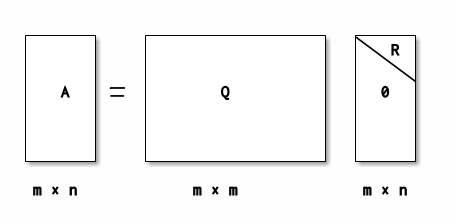
\includegraphics[width=.9\linewidth]{./figure5-1.png}
\caption{5.1. QR分解の抽象図}
\end{figure}

 Aの列の直交化に対応するQの部分のみを用いる代替手段は分解を行う際にしばしば有用である。(Figure 5.2.)\\
 この薄いQR分解は \(\bm{Q} = (\bm{Q}_1\bm{Q}_2)\ where\ \bm{Q}_1\ \in\ \mathbb{R}^{m\times n}\) に分割することで行われる。 \(\bm{Q}_2\) が0に掛けられても 0 となることに注意しなければならない。\\

\begin{figure}[htbp]
\centering
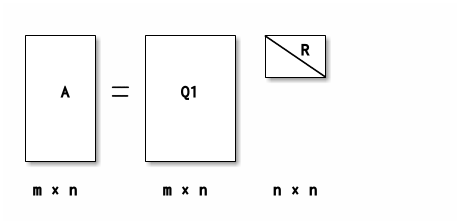
\includegraphics[width=.9\linewidth]{./figure5-2.png}
\caption{5.2 薄いQR展開 \(\bm{A} = \bm{Q}_1\bm{R}\)}
\end{figure}

\begin{align}
\bm{A} = (\bm{Q}_1\bm{Q}_2)\begin{pmatrix}\bm{R}\\0\end{pmatrix}=\bm{Q}_1\bm{R}
\tag{5.2}
\end{align}

 この方程式から、 \(\bm{R}(\bm{A})=\bm{R}(\bm{Q}_1)\) がわかる。このようにして、値空間 \(\bm{R(A)}\) の直交基底を計算した。さらに、(5.2) において j 列 を書き出すと、\\

\begin{align*}
\bm{a}_j = \bm{Q}_1\bm{r}_j = \Sigma^j_{i = 1}r_{ij}\bm{q}_i
\end{align*}

 \(\bm{R}\) の j 列は直交基底の \(\bm{a}_j\) の位置を保持することがわかります。\\
\end{frame}

\begin{frame}[fragile,label={sec:orgc28776f}]{例5.2 単純な数を用いたQR分解}
 \begin{columns}
\begin{column}{0.23\columnwidth}
\begin{block}{Octave Code}
\begin{minted}[frame=lines,linenos=true,obeytabs,tabsize=4]{octave}
A = [1 1 1;
     1 2 4; 
     1 3 9;
     1 4 16];
[Q,R] = qr(A)
\end{minted}
\end{block}
\end{column}

\begin{column}{0.73\columnwidth}
\begin{block}{Output}
\begin{verbatim}
Q =

  -0.50000   0.67082   0.50000   0.22361
  -0.50000   0.22361  -0.50000  -0.67082
  -0.50000  -0.22361  -0.50000   0.67082
  -0.50000  -0.67082   0.50000  -0.22361

R =

   -2.00000   -5.00000  -15.00000
    0.00000   -2.23607  -11.18034
    0.00000    0.00000    2.00000
    0.00000    0.00000    0.00000

\end{verbatim}
\end{block}
\end{column}
\end{columns}
\end{frame}

\begin{frame}[fragile,label={sec:orga4f64f1}]{例5.2 単純な数を用いたQR分解}
 薄いQR分解は \(qr(A,0)\) コマンドで実行する。\\
\begin{columns}
\begin{column}{0.3\columnwidth}
\begin{block}{Octave Code}
\begin{minted}[frame=lines,linenos=true,obeytabs,tabsize=4]{octave}
A = [1 1 1;
     1 2 4; 
     1 3 9;
     1 4 16];
[Q,R] = qr(A,0)
\end{minted}
\end{block}
\end{column}
\begin{column}{0.65\columnwidth}
\begin{block}{Output}
\begin{verbatim}
Q =

  -0.50000   0.67082   0.50000
  -0.50000   0.22361  -0.50000
  -0.50000  -0.22361  -0.50000
  -0.50000  -0.67082   0.50000

R =

   -2.00000   -5.00000  -15.00000
    0.00000   -2.23607  -11.18034
    0.00000    0.00000    2.00000

\end{verbatim}
\end{block}
\end{column}
\end{columns}
\end{frame}
\section{最小二乗問題の解き方}
\label{sec:org47d60f5}
\begin{frame}[allowframebreaks]{最小二乗問題}
 QR分解を用いて、以下の最小二乗問題を正規方程式を形成することなく解くことが出来る。これを行うために、ユークリッドベクトルノルムは直交変換の元で変わらないという事実を利用する。\\
\begin{align}
\min_{x}||\bm{b}-\bm{A}\bm{x}||_2&&where\ \bm{A}\ \in\ \mathbb{R}^{m\times n},\ m\geq n
\tag{5.3}
\end{align}
\begin{align*}
||\bm{Q}\bm{y}||_2=||\bm{y}||_2  
\end{align*}

\begin{columns}
\begin{column}{1.00\columnwidth}
\begin{block}{正規方程式}
\begin{align*}
\bm{A}^T\bm{A}\bm{x} = \bm{A}^T\bm{b}
\end{align*}
\end{block}
\end{column}
\end{columns}
\end{frame}

\begin{frame}[allowframebreaks]{}
 残差ベクトルに A についてのQR分解を用いて、\\
\begin{align*}
||\bm{r}||_2^2&=||\bm{b}-\bm{A}\bm{x}||_2^2=||\bm{b}-\bm{Q}\begin{pmatrix}\bm{R}\\0\end{pmatrix}\bm{x}||^2_2 \\
&=||\bm{Q}(\bm{Q}^T\bm{b}-\begin{pmatrix}\bm{R}\\0\end{pmatrix}\bm{x})||^2_2=||\bm{Q}^T\bm{b}-\begin{pmatrix}\bm{R}\\0\end{pmatrix}\bm{x}||^2_2
\end{align*}
 ここで \(\bm{Q}=(\bm{Q}_1\ \bm{Q}_2),\ where\ \bm{Q}_1\ \in\ \mathbb{R}^{m\times n}\) と分割して以下の式を導く。\\
 \begin{align*}
\bm{Q}^T\bm{b}=\begin{pmatrix}\bm{b}_1\\\bm{b}_2\end{pmatrix}:=\begin{pmatrix}\bm{Q}^T_1\bm{b}\\\bm{Q}^T_2\bm{b}\end{pmatrix}
\end{align*}
 即ち残差ベクトルの式は以下のように変形できる。\\
\begin{align}
||\bm{r}||^2_2=||\begin{pmatrix}\bm{b}_1\\\bm{b}_2\end{pmatrix}-\begin{pmatrix}\bm{R}\bm{x}\\0\end{pmatrix}||^2_2=||\bm{b}_1-\bm{R}\bm{x}||^2_2+||\bm{b}_2||^2_2
\tag{5.4}
\end{align}

 さらに A が線形独立であると仮定した場合、以下の式を満たす値を求めることで \(||\bm{r}||_2\) を最小化する値を求めることが出来る。\\
\begin{align*}
\bm{R}\bm{x}=\bm{b}_1
\end{align*}
 ここで次の定理が成り立つことになる。\\

\begin{block}{定理 5.3 QR分解を用いた最小二乗法の解}
 列についてフルランクであり、QR分解によって \(\bm{A}=\bm{Q}_1\bm{R}\) となる行列 \(\bm{A}\ \in\ \mathbb{R}^{m\times n}\) の最小二乗問題 \(min_x||\bm{A}\bm{x}-\bm{b}||_2\) は以下の唯一解を持つ。\\
\begin{align*}
\bm{x}=\bm{R}^{-1}\bm{Q}_1^T\bm{b}
\end{align*}
\end{block}
\end{frame}
\begin{frame}[fragile,label={sec:org2785add}]{例5.4 QR分解を用いて最小二乗問題を解く}
  尚 MATLAB では \(x=A\backslash b\) とすると同じアルゴリズムで解を求める。\\
\begin{columns}
\begin{column}{0.23\columnwidth}
\begin{block}{Octave Code}
\begin{minted}[frame=lines,linenos=true,obeytabs,tabsize=4]{octave}
A = [1 1;
     1 2; 
     1 3;
     1 4;
     1 5];
b = [7.9700;
     10.2000;
     14.2000;
     16.0000;
     21.2000];
# thin QR
[Q1,R]=qr(A,0)
x=R\(Q1'*b)
\end{minted}
\end{block}
\end{column}

\begin{column}{0.73\columnwidth}
\begin{block}{Output}
\begin{verbatim}
Q1 =
  -4.4721e-01  -6.3246e-01
  -4.4721e-01  -3.1623e-01
  -4.4721e-01   2.7756e-17
  -4.4721e-01   3.1623e-01
  -4.4721e-01   6.3246e-01
R =
  -2.23607  -6.70820
   0.00000   3.16228
x =
   4.2360
   3.2260
\end{verbatim}
\end{block}
\end{column}
\end{columns}
\end{frame}
\end{document}
